\documentclass[10pt, xcolor=table]{beamer}
\usepackage{inputenc}
\usepackage{graphicx}
\usepackage {mathtools}
\usetheme{CambridgeUS}
\usecolortheme{dolphin}
\usepackage{booktabs}
\usepackage{lscape}
\usepackage{caption}
\usepackage{tikz}
\usepackage{subcaption}
\usepackage{multicol}
\usepackage{xcolor}
\usepackage{pgfplots}
\usepackage{bm}
\usepackage{multicol}
\usepackage{adjustbox}
\usepackage{multicol}



\newcommand\dc[1]{\textcolor{blue}{#1}}
\setcounter{tocdepth}{3}
\pgfplotsset{compat=1.18}
\usepgfplotslibrary{external} 
\tikzexternalize

\newlength\figureheight
\newlength\figurewidth

\definecolor{myNewColorA}{RGB}{7,47,95}
\definecolor{myNewColorB}{RGB}{210,50,35}
\definecolor{myNewColorC}{RGB}{244,182,0}
\definecolor{myNewColorD}{RGB}{85,168,104}

\setbeamercolor*{palette primary}{bg=myNewColorC}
\setbeamercolor*{palette secondary}{bg=myNewColorB, fg=white}
\setbeamercolor*{palette tertiary}{bg=myNewColorA, fg=white}
\setbeamercolor*{titlelike}{fg=myNewColorA}
\setbeamercolor*{title}{bg=myNewColorA, fg=white}
\setbeamercolor*{item}{fg=myNewColorA}
\setbeamercolor*{caption name}{fg=myNewColorA}

\usefonttheme{professionalfonts}




\usepackage{natbib}
\usepackage{hyperref}
%------------------------------------------------------------
\titlegraphic{
    \begin{figure}
        \centering
        \begin{subfigure}[l]{0.45\textwidth}
            \centering
            
\includegraphics[width=2.5cm,height=1.5cm]{images/Logo_U.T.P.png}
        \end{subfigure}
        \hfill
        \begin{subfigure}[r]{0.45\textwidth}
            \centering
            
\includegraphics[width=2.5cm,height=2.5cm]{images/logo-maestria-scaled.jpg}
        \end{subfigure}
    \end{figure}
}

\setbeamerfont{title}{size=\Large\bfseries}
\setbeamerfont{subtitle}{size=\small}
\setbeamerfont{author}{size=\small}
\setbeamerfont{institute}{size=\footnotesize}

\title[Universidad Tecnológica de Pereira]{Chained Gaussian Processes for Hydrological Forecasting}


 
\author[Julián David Pastrana-Cortés et al.]{%
	\texorpdfstring{
		\begin{tabular}{c}
			Julián David Pastrana-Cortés \\[1.5mm]
			\textit{Director: Álvaro Angel Orozco-Gutiérrez} \\[1.5mm]
			\textit{Co-director: David Augusto Cardenas-Peña} \\
		\end{tabular}
	}{Julián David Pastrana-Cortés et al.}
}



\institute[Automatic]{Automatic Research Group}
\date{\today}

\AtBeginSection[]{
  \begin{frame}
    \vfill
    \centering
    \begin{beamercolorbox}[sep=8pt,center,shadow=true,rounded=true]{title}
      \usebeamerfont{title}\insertsectionhead\par%
    \end{beamercolorbox}
    \vfill
  \end{frame}
}

%------------------------------------------------------------

\begin{document}

\frame{\titlepage}

\section*{Motivation}

\begin{frame}{Motivation}
  frame
\end{frame}


\begin{frame}{Objetive}
Develop a predictive methodology for thermoelectric plant dispatch based on historical data. This aims to estimate the natural gas demand for each plant within the planning horizon, leveraging hydrological forecasting for enhanced accuracy.

\begin{figure}
    \centering
    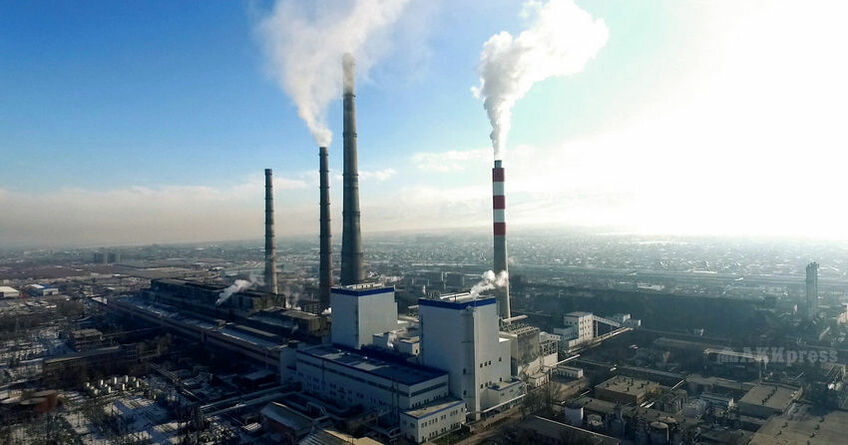
\includegraphics[width=\textwidth, height=5cm]{images/Bishkek-.jpeg}
\end{figure}
    
\end{frame}

\begin{frame}{}
    Modeling thermolectic time series is hard. Instead, model hydrological time series forecasting via hydrothermal dispatch, inferring thermoelectric dispatch.

\begin{figure}
    \centering
    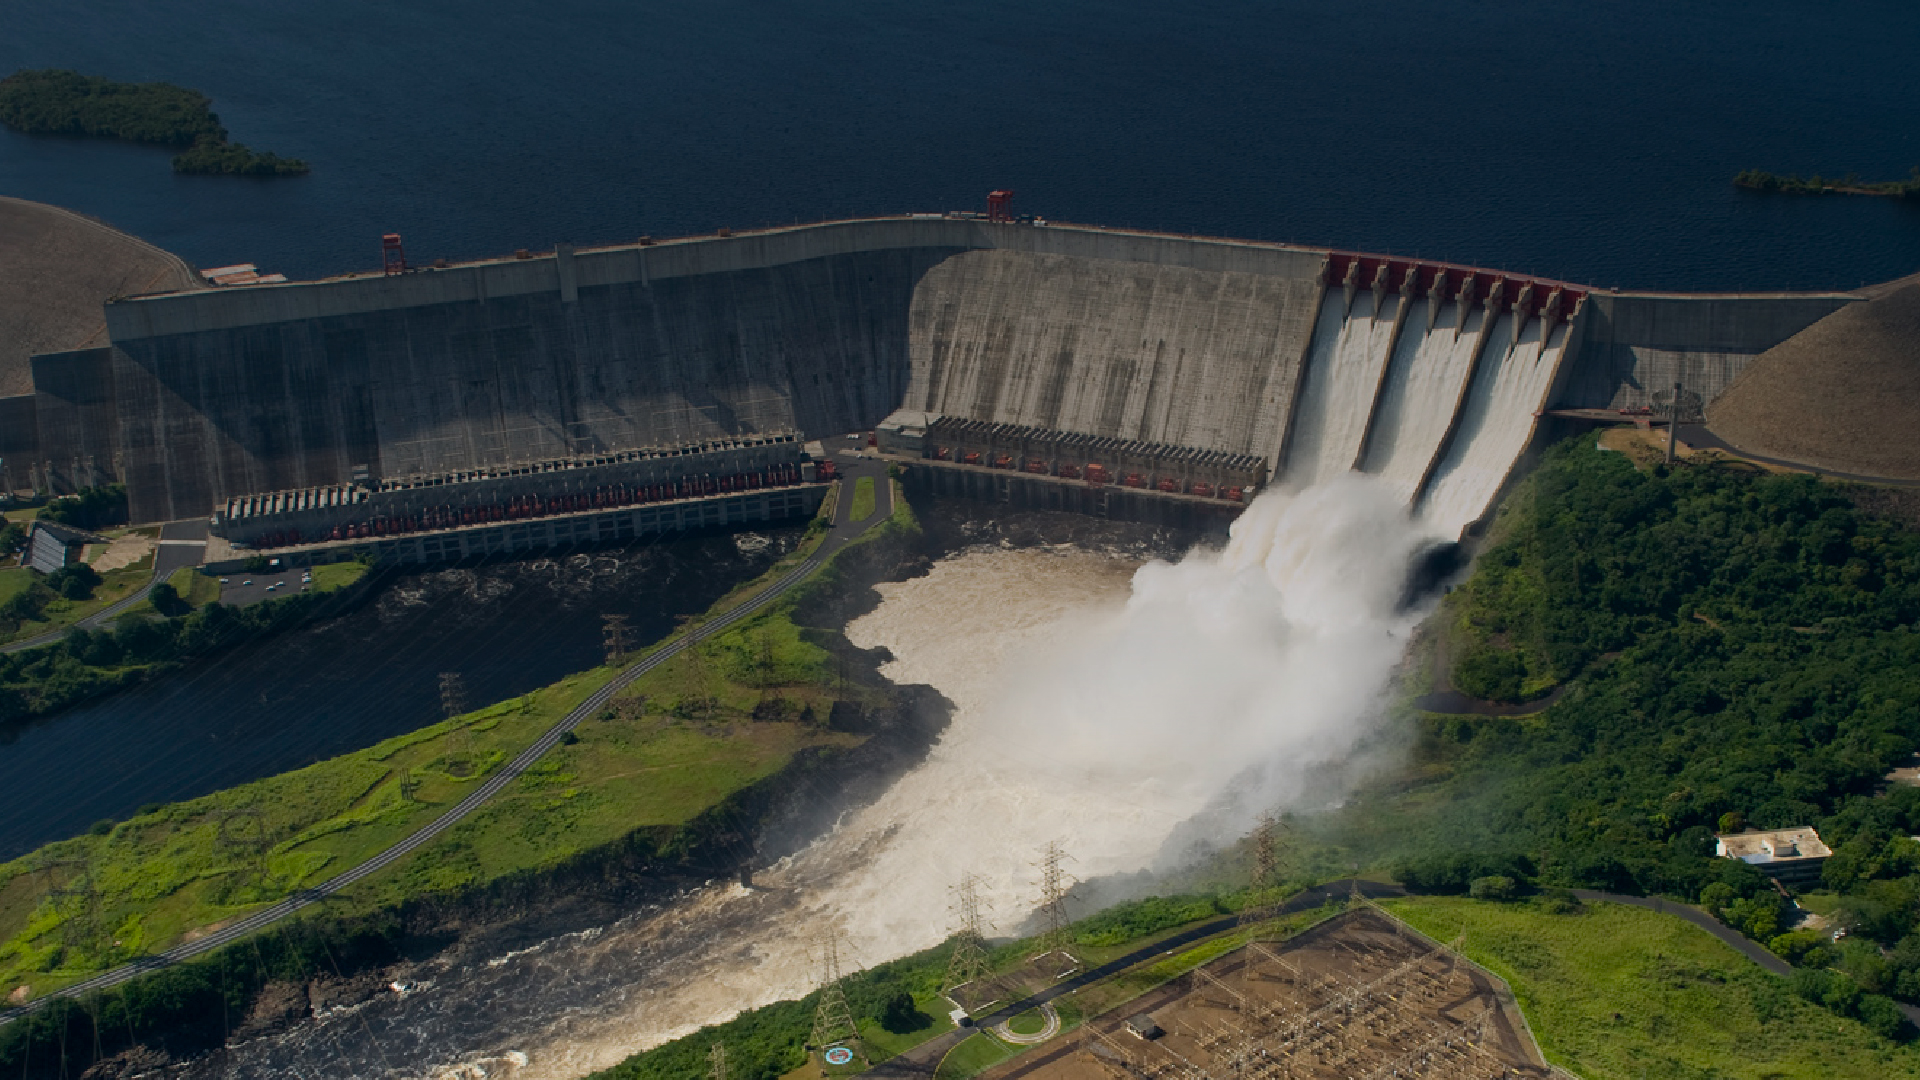
\includegraphics[width=\textwidth, height=5cm]{images/hydroelectric.jpg}
\end{figure}
\end{frame}



\begin{frame}{Motivation}
We want a non-linear model to not only forecast water resources but also provide a confidence interval that measures the certainty of that prediction.
\begin{figure}
     \centering
     \begin{subfigure}[b]{0.3\textwidth}
         \centering
         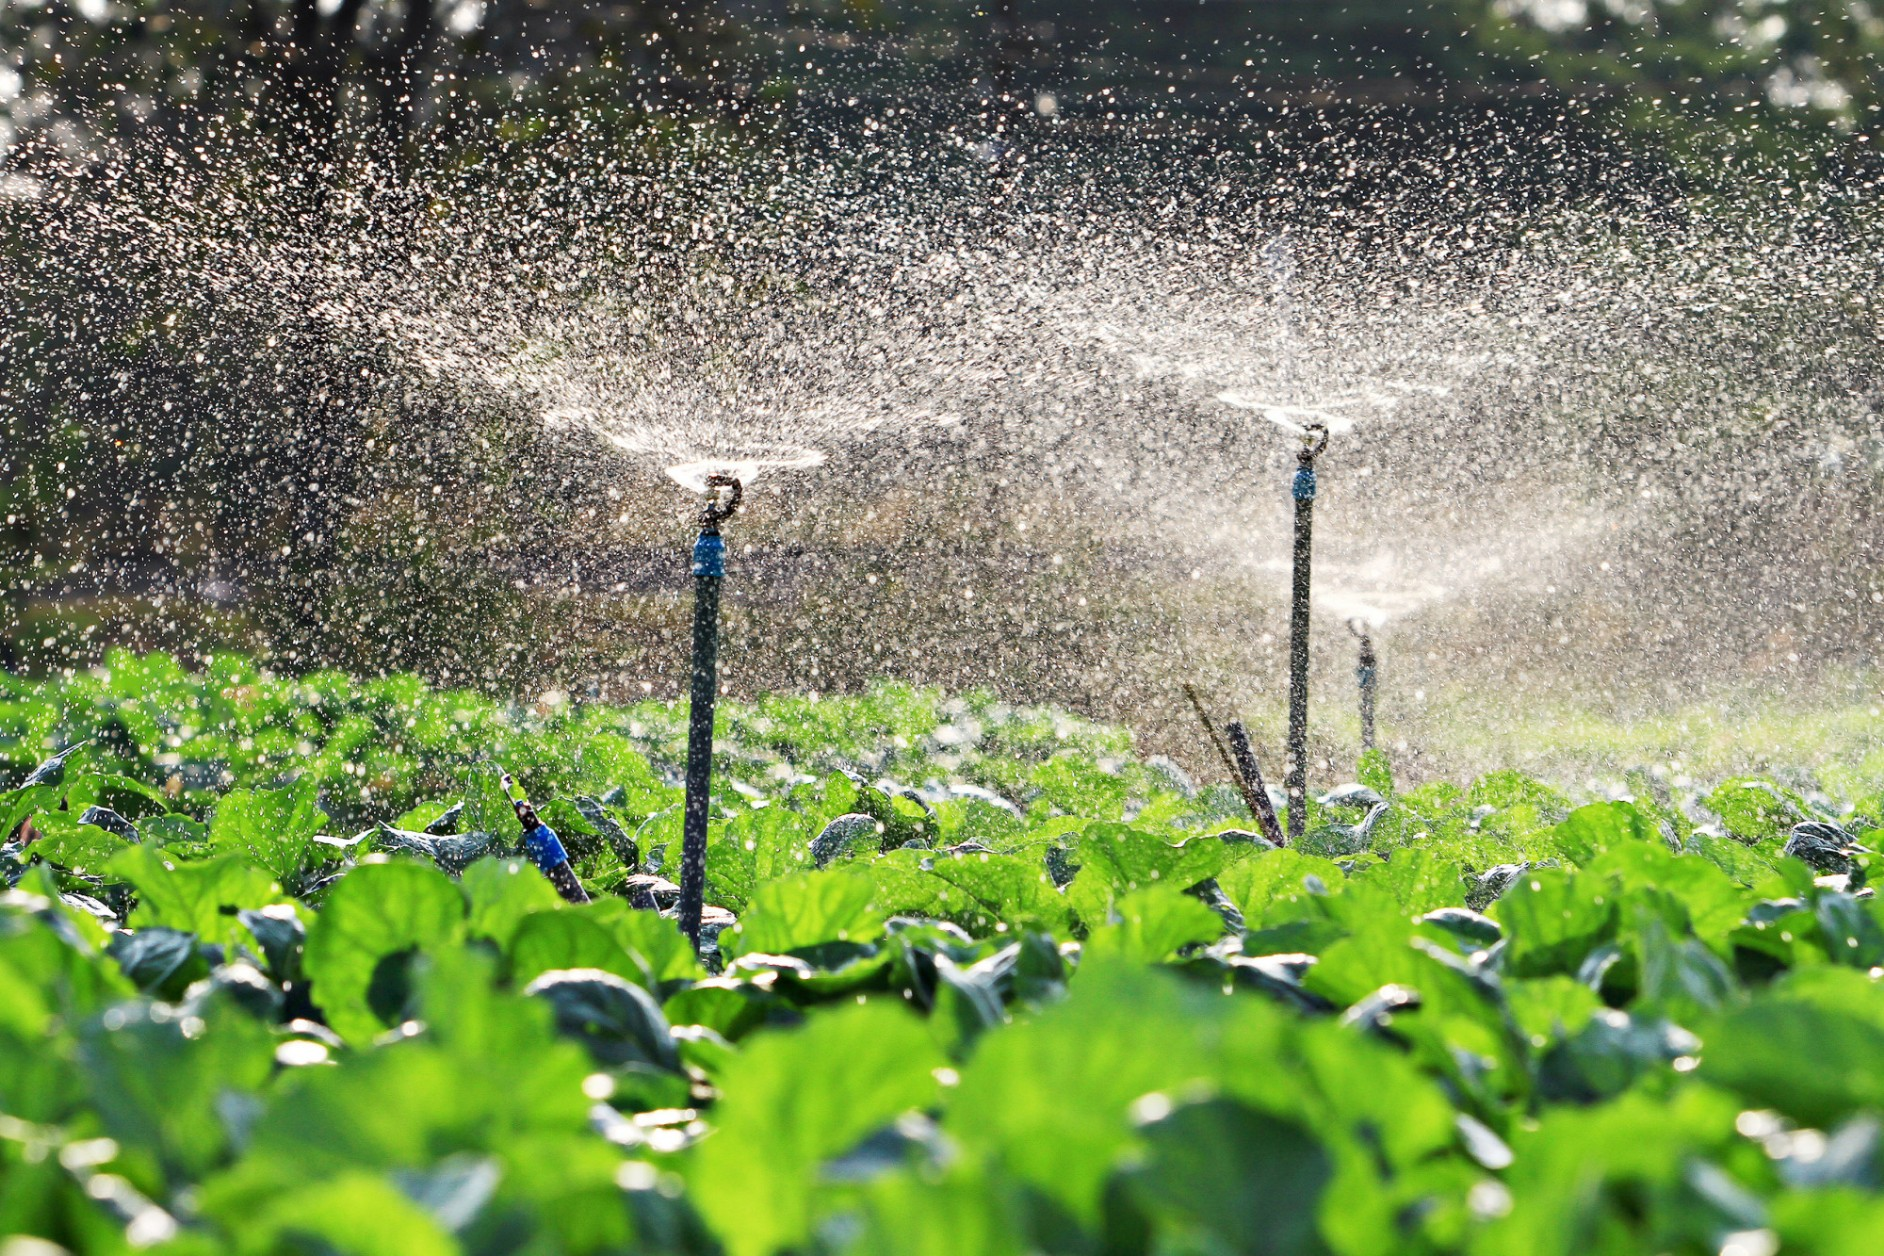
\includegraphics[width=\textwidth, height=4cm]{images/irrigation.jpg}
         \caption{Irrigation}
         \label{fig:y equals x}
     \end{subfigure}
     \hfill
     \begin{subfigure}[b]{0.3\textwidth}
         \centering
         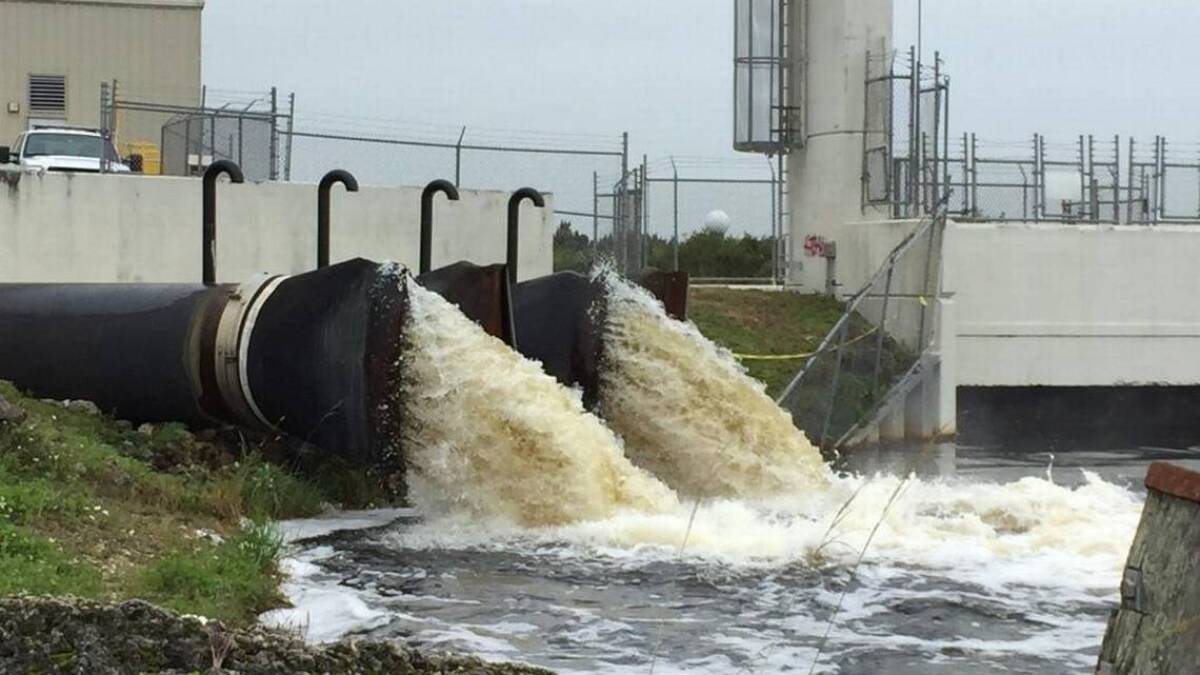
\includegraphics[width=\textwidth, height=4cm]{images/flood_control.jpeg}
         \caption{Flood control}
         \label{fig:three sin x}
     \end{subfigure}
     \hfill
     \begin{subfigure}[b]{0.3\textwidth}
         \centering
         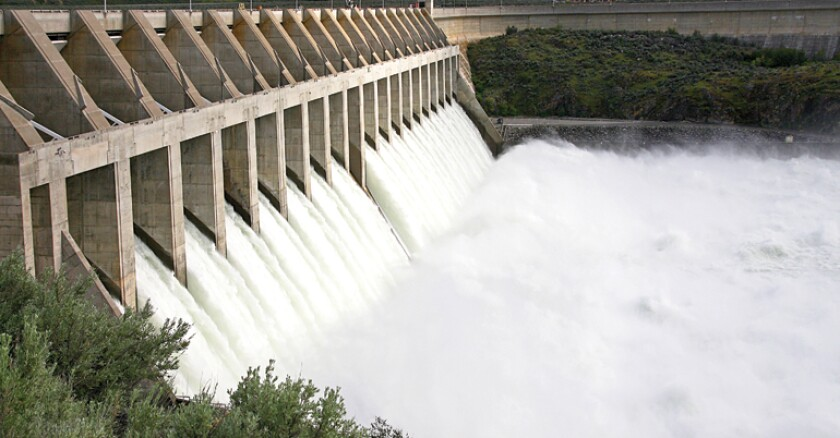
\includegraphics[width=\textwidth, height=4cm]{images/hydro_gen.jpeg}
         \caption{Hydropower generation}
         \label{fig:five over x}
     \end{subfigure}
\end{figure}

\textbf{Difficulties}: non-linearities, high stochasticity, and complex water resource patterns.

\end{frame}


\section*{Dataset}
\begin{frame}{Dataset Construction}
Consider $\mathbf{v}_{n} \in \mathbb{R}^{D+}$ as a value useful volume time series observed at time $n$ for all $D$ reservoirs. The dataset comprises $N$ pairs of input/output observations $\{\mathbf{x}_n, \mathbf{y}_n\}_{n=1}^N = \{\mathbf{X}, \mathbf{Y}\}$, defined as:

\begin{equation*}
    \mathbf{y}_n = \mathbf{v}_{n}, \quad \mathbf{x}_n = \mathbf{v}_{n-1}
\end{equation*}

Each $\mathbf{v}_n$ represents a realization of a random vector $\bm{y}$. Considering $\bm{y}(\bm{x})$ for some input space $\bm{x} \in \mathbf{\chi}$, we model a stochastic process.
\end{frame}

\section*{The Model}

\begin{frame}{Gaussian Process Framework}
A Gaussian Process (GP) models a collection of random variables, any finite number of which follow a joint Gaussian distribution:
\begin{equation*}
    \bm{f}(\mathbf{x}) \sim \mathcal{GP}(\mathbf{0}, \bm{k}(\mathbf{x}, \mathbf{x}'))
\end{equation*}
The covariance function $\bm{k}$ computes the correlation between points in the input space.
\end{frame}

\begin{frame}{Likelihood}
We model outcomes $\mathbf{y}(\mathbf{x})$ using parameters $\boldsymbol{\theta}_d(\mathbf{x})$ for each outcome $y_d(\mathbf{x})$. $\boldsymbol{\theta}(\mathbf{x})$ combines all parameters across outcomes. The likelihood, or chance of observing our data $\mathbf{y}(\mathbf{x})$, is calculated by multiplying the likelihoods of each outcome, as shown:
\begin{equation*}
    p(\mathbf{y}(\mathbf{x}) \mid \boldsymbol{\theta}(\mathbf{x})) = \prod_{d=1}^D p(y_{d}(\mathbf{x}) \mid \boldsymbol{\theta}_{d}(\mathbf{x}))
\end{equation*}
\end{frame}



\begin{frame}{Chained Gaussian Processes}
In each likelihood distribution, parameters $\theta_{d,j}(\mathbf{x})$ are derived from Gaussian Processes (GP), specifically, $\theta_{d,j}(\mathbf{x}) = g_{d,j}(f_{d,j}(\mathbf{x}))$. This means we transform GP outputs to obtain our parameters. Combining all transformed GP outputs, $\mathbf{f}(\mathbf{x})$, allows us to model the likelihood of our observations $\mathbf{y}(\mathbf{x})$ as:
\begin{equation*}
p(\mathbf{y}(\mathbf{x}) \mid \mathbf{f}(\mathbf{x})) = \prod_{d=1}^D p(y_{d}(\mathbf{x})\mid \mathbf{f}_{d}(\mathbf{x}))
\end{equation*}
Here, each $y_{d}(\mathbf{x})$ is assumed to follow a LogNormal distribution, ensuring positivity in our predictions.
\end{frame}


\section*{Results}

\begin{frame}{Forecasting}
    \begin{figure}
    \centering
    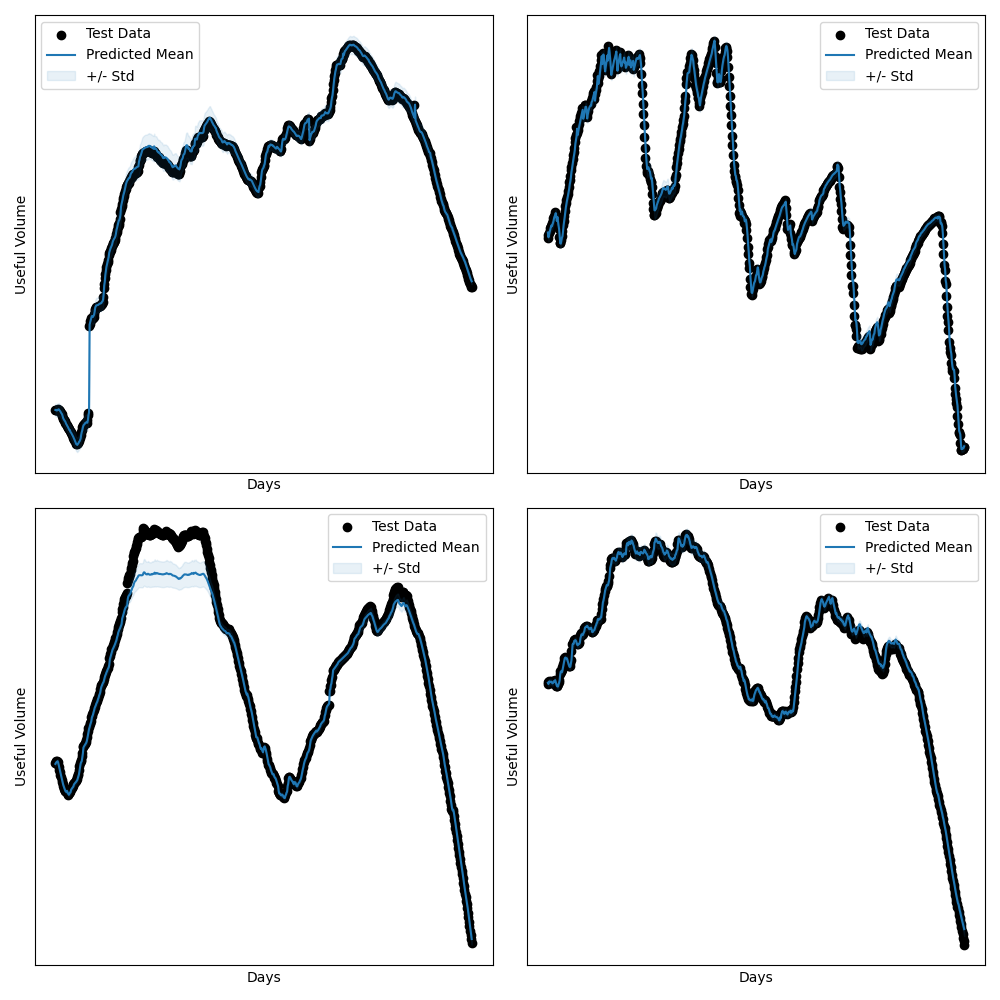
\includegraphics[width=0.7\textwidth, height=7.5cm]{images/predictions_test.png}
\end{figure}
\end{frame}





\begin{frame}{Thank You for Watching!}
\centering
\Large{Thank you for your attention!}\\
\vspace{10mm} % Adjust the space as needed
\large{Questions or Comments?}\\
\vspace{5mm} % Adjust the space as needed
\large{Feel free to reach out for further discussion.}
\end{frame}


\end{document}



